\chapter{两轮平衡车自主导航系统开发}

两轮平衡车自动行驶的实现依赖自主导航系统。该系统主要承担实时感知与路径规划任务：在接收到目标点信息后，结合定位数据与环境感知结果规划行驶路线，并将运动指令发送至控制系统，从而实现自动行驶。本章首先根据需求搭建自主导航系统硬件环境，随后完成软件部分开发。

\section{自主导航系统的设计}

自主导航系统的结构如图\ref{自主导航系统总体设计}所示，整体由主控计算单元、传感器与信号转换模块、通信连接模块、电源模块四部分构成。

\begin{figure}[htbp]
\centering
\includesvg[width=5.76806in,height=1.60139in]{figures/chapter04/自主导航系统总体设计}
\caption{自主导航系统总体设计}
\label{自主导航系统总体设计}
\end{figure}

自主导航系统以主控计算机为核心，采用通用数据接口连接多类传感器及信号转换模块，实现对定位信息与环境感知信息的统一接收与处理。系统同时集成无线通信与可视化交互模块，能够远程接收用户终端的控制指令，并实时展示系统运行状态。在导航执行过程中，主控计算机周期性地下发路径规划模块生成的运动指令，同时采集来自控制系统的反馈信息，构成闭环控制体系，确保导航系统的实时性、稳定性与安全性。

\section{自主导航系统的硬件环境搭建}

根据自主导航系统的总体设计，对硬件进行选型，设计连接电路并实际搭建自主导航系统的硬件环境。

\subsection{自主导航系统的硬件选型}



为满足系统对高精度、高更新率定位的需求，选用北天 BT‑982K3 双天线 RTK GNSS 模块。该模块支持 GPS、北斗等多星系统，具备20Hz实时RTK定位能力。在合理布设双天线的条件下，可实现优于2\,cm的平面定位精度和0.1°/1\,m的航向精度。

为实现近距离障碍物检测，系统配置电应普 DYP-A21 型超声波雷达。该雷达测距范围为3cm--500cm。在量程设定为200cm的条件下，模块响应时间小于200ms，能够满足低速移动场景中的动态障碍物感知需求。结合一拖四转接模组，本系统部署4个超声波传感器，形成前后左右覆盖的近场检测布局，有效提升环境安全性与避障可靠性。

视觉感知需满足对中近距离障碍物的深度估计要求，因此相机应具备合理的基线长度与足够的视场角。较长的基线有利于感知较远（15m）的深度，而适中的视场角有助于覆盖小车前方主要作业区域，提升环境感知完整性。本系统选用DECXIN‑2M‑SM‑2782V1双目相机，其12\,cm基线与92°视场角在精度与视野覆盖之间取得良好平衡。该相机支持1600×1200@60FPS的同步图像输出，满足实时立体匹配与图像处理的计算需求。

为满足系统在视觉感知、深度估计与路径规划等任务中的高并发计算需求，主控平台选用 NVIDIA Jetson Orin Nano Super。该模块内置基于Ampere架构的 GPU，具1024个CUDA核心与32个张量核心，AI算力可达67 TOPS，适用于多路神经网络的实时推理处理。同时，配备六核 Cortex-A78AE CPU 与 8GB LPDDR5 高带宽内存（102 GB/s），支持高帧率图像与多传感器数据的同步处理。此外，其丰富的接口（包括 MIPI CSI、USB 3.2、PCIe Gen3 x4 等）便于与相机、定位与控制模块集成。

\subsection{硬件线路连接}

分析自主导航系统硬件供电需求可知，主控电脑需要19V DC电源供电，而传感器及信号转换元件等需要5V DC电源供电，电路连接如图\ref{自主导航系统电源模块}所示。

以24V直流电池电源为基础，通过24V-220V逆变器将24V直流电转换为220V交流电后，分别采用19V和12V电源适配器为主控电脑及外部设备提供所需电压。其中，19V电源适配器为主控电脑供电，12V电源适配器则为USB拓展坞供能。USB拓展坞进一步将12V电压转换为5V，并通过各类接口为USB-485转换器、IMU、超声波雷达转接模组、双目相机、GPS及便携无线路由网卡等多种外部设备提供稳定的电源与数据连接。

\begin{figure}[htbp]
\centering
\includesvg[width=4.77083in,height=2.41667in]{figures/chapter04/自主导航系统电源模块}
\caption{自主导航系统电源模块}
\label{自主导航系统电源模块}
\end{figure}

自主导航系统的信号连接如图\ref{自主导航系统信号电路连接}所示。主控电脑作为核心处理单元，通过多个USB接口与双目相机、IMU、GPS等传感与通信设备进行数据交互。其中，双目相机直接连接主控电脑以保证带宽和实时性，其他设备则通过USB拓展坞接入，以提升接口扩展能力。此外，主控电脑通过USB-485转换器将USB信号转换为RS-485信号，进而连接超声波雷达转接模块，实现对多路超声波雷达（UART接口）的统一管理与数据采集。同时，主控电脑通过以太网口与控制系统STM32F407微控制器通信，完成自主导航系统与控制系统之间的信息交互。上述信号连接设计有效整合了各类传感器与执行单元，保障了数据传输的实时性与稳定性。

\begin{figure}[htbp]
\centering
\includesvg[width=5.76806in,height=2.58611in]{figures/chapter04/自主导航系统信号连接}
\caption{自主导航系统信号电路连接}
\label{自主导航系统信号电路连接}
\end{figure}

自主导航系统硬件平台实物如图\ref{自主导航系统硬件平台实物图}所示。

\begin{figure}[htbp]
\centering
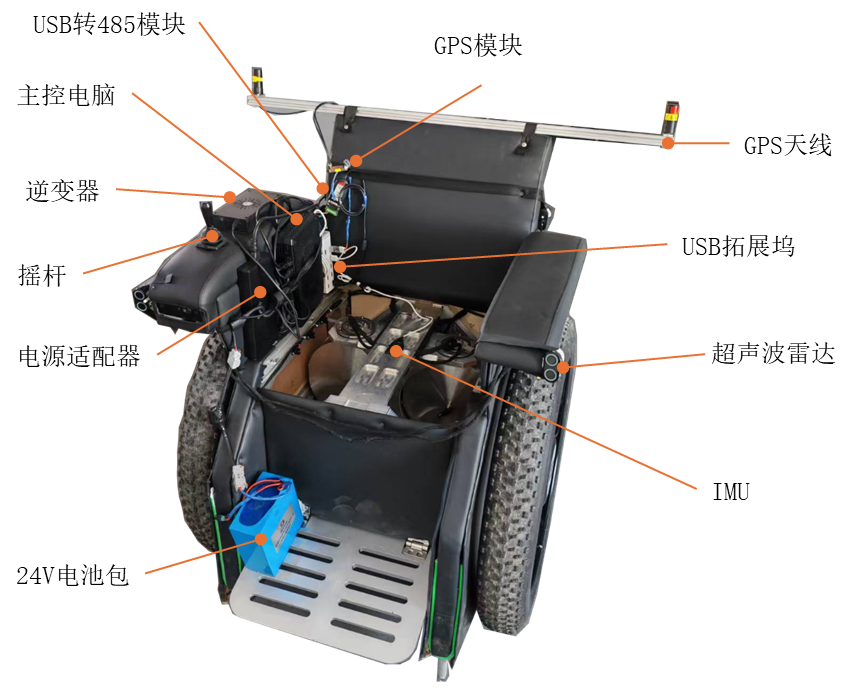
\includegraphics[width=4.52308in,height=3.65878in]{figures/chapter04/自主导航系统硬件平台实物图.png}
\caption{自主导航系统硬件平台实物图}
\label{自主导航系统硬件平台实物图}
\end{figure}

\section{自主导航系统的软件开发}

自主导航系统是实现两轮平衡车自动行驶的核心模块之一。该系统承上启下，既需准确获取环境与自身状态信息，又需据此完成路径规划与任务执行。自主导航系统软件结构如图\ref{自主导航系统软件结构}所示，整体划分为地图模块、定位模块、感知模块、通讯模块、交互模块与主控模块六大部分。

\begin{figure}[htbp]
\centering
\includesvg[width=5.76806in,height=2.67083in]{figures/chapter04/自主导航系统软件结构}
\caption{自主导航系统软件结构}
\label{自主导航系统软件结构}
\end{figure}

各模块功能如下。主控模块作为系统中枢，负责整合各类信息，执行路径规划、任务管理与控制指令下发，并包含导航子模块与日志子模块，分别用于路径决策与运行数据记录。地图模块提供静态环境空间信息，包括基础地图与代价图，为路径规划提供空间依据。定位模块融合轮速计、IMU与GPS等多源信息，实现车体全局位姿的持续估计，兼顾局部短时精度与长期漂移补偿。感知模块结合双目相机和超声波传感器获取环境信息。通讯模块完成与下位机的信息交互，上行包括轮速计数据、控制状态等反馈，下行为运动指令的周期性下发。交互模块面向人机交互需求，既包括开发调试阶段使用的可视化工具（如RViz），也包括面向用户的小程序界面，用于设定目标和查看状态。

本系统采用机器人操作系统（Robot Operating System, ROS）作为系统软件架构的基础。ROS是一种开源的机器人软件开发平台，具有模块化、分布式、消息传递机制等特点，能够有效地支持机器人系统的快速开发与集成。ROS通过节点（Node）、主题（Topic）、服务（Service）等通信机制，便于各功能模块的解耦与协作，提高了系统的可扩展性与维护性。

地图模块方面，为实现自主导航功能，需先获取车辆运行环境的静态地图。系统对测试场地进行测绘并制作静态地图。该地图作为导航与路径规划的基础数据，已集成至ROS环境，供后续模块调用。

通讯模块方面，系统通过UDP协议与下位机进行数据交互。上位机（ROS主控端）将速度、角速度等运动指令实时发送至下位机，以驱动控制系统；下位机将控制状态、传感器数据等反馈信息返回上位机，实现闭环控制与状态监测。UDP协议传输效率高、实时性好，能够满足车辆控制系统对时延的要求。

\begin{figure}[htbp]
\centering
\subfigure[RViz界面]{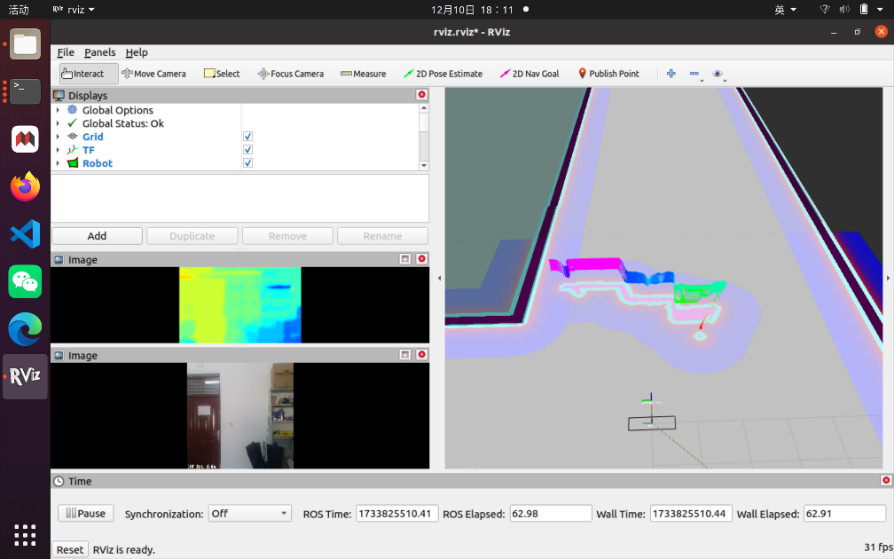
\includegraphics[width=0.62\textwidth]{figures/chapter04/RViz界面.png}}
\hfill
\subfigure[小程序界面\label{小程序界面}]{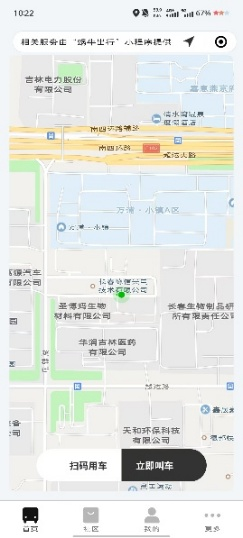
\includegraphics[width=0.20\textwidth]{figures/chapter04/小程序界面.jpeg}}
\caption{交互界面}
\end{figure}

交互模块如图\ref{小程序界面}所示。系统选用RViz作为主要可视化开发与测试工具。RViz是ROS中的三维可视化平台，既可实现外部信息的图形化显示，也可用于发布控制信息，从而实现对机器人的监测与控制。通过RViz可直观展示车辆在地图中的位置、运动轨迹及传感器数据，便于开发人员调试与功能验证。此外，为实现与用户端（如手机小程序）的实时交互，系统采用MQTT协议进行加密通信。上位机可通过MQTT协议将车辆当前位置等状态信息实时发送至小程序端，用户亦可通过小程序下发目的地指令，系统接收后自动执行目标导航。该设计有效提升了系统的人机交互能力与操作便利性。

\subsection{定位模块}

在公园、封闭社区等典型应用场景中，由于环境结构复杂、遮挡物较多，单一传感器往往难以实现稳定、连续的高精度定位。为了克服这一问题，本系统定位模块基于多传感器融合策略进行设计，主要集成了GPS、IMU以及轮速传感器，并采用卡尔曼滤波算法对多源信息进行时序融合，以提升系统的定位鲁棒性与精度。

不同传感器具有各自的优势与局限性。GPS可提供全局坐标系下的绝对位置，具备长期定位的能力，但其更新率较低，且在建筑物遮挡或室内环境下易发生信号中断；IMU可高频采集加速度与角速度数据，适合用于姿态估计和短时运动推算，但受限于积分误差的累积，存在长期漂移问题；轮速传感器能够精确测量轮子线速度，但在出现打滑等工况时，其测量结果将偏离实际情况，无法独立支撑完整定位。

针对以上特性，本定位模块以IMU构建高频运动预测模型，在每个时间步中基于当前姿态估计与速度信息进行状态预测；引入轮速传感器的观测数据周期性修正线速度估计，进而抑制IMU短期内的积分漂移；GPS作为低频全局观测源，用于修正整体位置估计的长期偏移。在此基础上，卡尔曼滤波框架通过预测---修正的迭代机制，有效融合上述信息，提升定位系统的稳定性和抗干扰能力。

\subsubsection{定位模块的设计}

本模块的整体运行流程如图\ref{定位模块流程图}所示，根据卡尔曼滤波的原理，设计主要包括系统初始化、时间更新、观测更新等步骤。

系统启动后，首先完成传感器驱动和状态矩阵的初始化，随后进入主循环。在循环中，系统基于时间更新周期与观测更新周期交替驱动状态估计与输出控制。

在每个时间更新周期到达时，系统首先读取IMU与轮速传感器数据，利用运动模型进行一次状态预测，用于推算车辆当前位置、姿态角和线速度。该步骤提供连续且高频的状态输出。

接着系统判断是否到达观测更新周期。若尚未到达，则进入下一轮时间更新；若已经到达，则进一步读取GPS数据，并对其信号质量进行判断。如果GPS质量满足设定阈值，系统会基于GPS信息执行观测修正，从而校正状态预测中的累积误差；若GPS质量较差或信号丢失，则跳过修正，直接维持预测状态。

无论是否执行观测修正，系统都会将当前状态中的位姿信息输出至主控模块，包括车辆的位置、速度和姿态角等关键参数。通过该机制，主控模块可按固定频率获得融合估计后的状态信息，确保导航与控制任务的连续性和一致性。

\begin{figure}[htbp]
\centering
\includesvg[width=5.58333in,height=4.83333in]{figures/chapter04/定位模块流程图}
\caption{定位模块流程图}
\label{定位模块流程图}
\end{figure}

两种周期交替作用，确保了系统在不同精度与频率层次上的信息融合。时间更新周期以高频率提供连续、平滑的状态估计；观测更新周期以低频率提供全局位置校准，从而实现系统在动态环境中的高鲁棒性和精度保持。

\subsubsection{卡尔曼融合定位的实现}

卡尔曼滤波推算车辆状态分为两个步骤：时间更新和观测更新。滤波器通过这两个步骤融合传感器观测与模型预测，从而优化状态估计。

状态向量 \(x_{k}\) 包含9个状态量：
\begin{equation}
x_{k} = \begin{bmatrix}
p_{x} & p_{y} & p_{z} & v_{x} & v_{y} & v_{z} & a_{x} & a_{y} & a_{z}
\end{bmatrix}^{T}
\end{equation}

式中
\emph{p\textsubscript{x}}，\emph{p\textsubscript{y}}，\emph{p\textsubscript{z}}------GPS坐标；

\emph{a\textsubscript{x}}，\emph{a\textsubscript{y}}，\emph{a\textsubscript{z}}------IMU加速度；

\emph{v\textsubscript{x}}，\emph{v\textsubscript{y}}，\emph{v\textsubscript{z}}------轮速传感器推算线速度。

时间更新（预测）步骤通过动力学模型对下一时刻的状态进行估计。
\begin{equation}
\begin{array}{r}
x_{k + 1} = F_{k}x_{k} + B_{k}u_{k} + w_{k}
\end{array}
\end{equation}

式中
\emph{F\textsubscript{k}}------状态转移矩阵，用于从当前状态推算下一时刻的状态；

\emph{B\textsubscript{k}}------控制输入矩阵（设为零）；

\emph{u\textsubscript{k}}------外部输入控制（设为零）；

\emph{w\textsubscript{k}}------过程噪声，假设为零均值高斯噪声，协方差为\emph{Q\textsubscript{k}}。

状态转移矩阵\emph{F\textsubscript{k}}可以基于车辆的运动模型写成：
\begin{equation}
\begin{array}{r}
F_{k} = \begin{bmatrix}
1 & 0 & 0 & \Delta t & 0 & 0 & \frac{1}{2}\Delta t^{2} & 0 & 0 \\
0 & 1 & 0 & 0 & \Delta t & 0 & 0 & \frac{1}{2}\Delta t^{2} & 0 \\
0 & 0 & 1 & 0 & 0 & \Delta t & 0 & 0 & \frac{1}{2}\Delta t^{2} \\
0 & 0 & 0 & 1 & 0 & 0 & \Delta t & 0 & 0 \\
0 & 0 & 0 & 0 & 1 & 0 & 0 & \Delta t & 0 \\
0 & 0 & 0 & 0 & 0 & 1 & 0 & 0 & \Delta t \\
0 & 0 & 0 & 0 & 0 & 0 & 1 & 0 & 0 \\
0 & 0 & 0 & 0 & 0 & 0 & 0 & 1 & 0 \\
0 & 0 & 0 & 0 & 0 & 0 & 0 & 0 & 1
\end{bmatrix}
\end{array}
\end{equation}

式中------\(\Delta t\)为采样时间。

预测的协方差矩阵更新公式为：
\begin{equation}
\begin{array}{r}
P_{k + 1} = F_{k}P_{k}{F_{k}}^{T} + Q_{k}
\end{array}
\end{equation}

过程噪声协方差矩阵\(Q_{k}\)设为：
\begin{equation}
\begin{array}{r}
\  \\
Q_{k} = \begin{bmatrix}
\frac{0.25\Delta t^{3}}{3} & 0 & 0 & \frac{0.25\Delta t^{2}}{2} & 0 & 0 & 0.25\Delta t & 0 & 0 \\
0 & \frac{0.25\Delta t^{3}}{3} & 0 & 0 & \frac{0.25\Delta t^{2}}{2} & 0 & 0 & 0.25\Delta t & 0 \\
0 & 0 & \frac{0.25\Delta t^{3}}{3} & 0 & 0 & \frac{0.25\Delta t^{2}}{2} & 0 & 0 & 0.25\Delta t \\
\frac{0.25\Delta t^{2}}{2} & 0 & 0 & 0.01\Delta t & 0 & 0 & 0 & 0 & 0 \\
0 & \frac{0.25\Delta t^{2}}{2} & 0 & 0 & 0.01\Delta t & 0 & 0 & 0 & 0 \\
0 & 0 & \frac{0.25\Delta t^{2}}{2} & 0 & 0 & 0.01\Delta t & 0 & 0 & 0 \\
0.25\Delta t & 0 & 0 & 0 & 0 & 0 & 0.25 & 0 & 0 \\
0 & 0.25\Delta t & 0 & 0 & 0 & 0 & 0 & 0.25 & 0 \\
0 & 0 & 0.25\Delta t & 0 & 0 & 0 & 0 & 0 & 0.25
\end{bmatrix}
\end{array}
\end{equation}

观察更新步骤结合传感器观测值来修正预测状态。假设测量模型为线性的：
\begin{equation}
\begin{array}{r}
z_{k} = H_{k}x_{k} + v_{k}
\end{array}
\end{equation}

式中
\emph{z\textsubscript{k}}------测量值向量（GPS位置、IMU加速度和轮速推算的速度）；

\emph{H\textsubscript{k}}------测量矩阵，它将状态向量映射到测量空间,H\emph{\textsubscript{k}}=E；

\emph{v\textsubscript{k}}------测量噪声。

测量噪声协方差\emph{R\textsubscript{k}}为：
\begin{equation}
\begin{array}{r}
R_{k} = \begin{bmatrix}
25 & 0 & 0 & 0 & 0 & 0 & 0 & 0 & 0 \\
0 & 25 & 0 & 0 & 0 & 0 & 0 & 0 & 0 \\
0 & 0 & 25 & 0 & 0 & 0 & 0 & 0 & 0 \\
0 & 0 & 0 & 0.01 & 0 & 0 & 0 & 0 & 0 \\
0 & 0 & 0 & 0 & 0.01 & 0 & 0 & 0 & 0 \\
0 & 0 & 0 & 0 & 0 & 0.01 & 0 & 0 & 0 \\
0 & 0 & 0 & 0 & 0 & 0 & 0.0025 & 0 & 0 \\
0 & 0 & 0 & 0 & 0 & 0 & 0 & 0.0025 & 0 \\
0 & 0 & 0 & 0 & 0 & 0 & 0 & 0 & 0.0025
\end{bmatrix}
\end{array}
\end{equation}

更新步骤的卡尔曼增益为：
\begin{equation}
\begin{array}{r}
K_{k} = P_{k}{H_{k}}^{T}\left( H_{k}P_{k}{H_{k}}^{T} + R_{k} \right)^{- 1}
\end{array}
\end{equation}

状态更新：
\begin{equation}
\begin{array}{r}
x_{k} = x_{k} + K_{k}\left( z_{k} - H_{k}x_{k} \right)
\end{array}
\end{equation}

协方差更新：
\begin{equation}
\begin{array}{r}
P_{k} = \left( I - K_{k}H_{k} \right)P_{k}
\end{array}
\end{equation}

\subsubsection{定位效果}

系统运行后，基于卡尔曼滤波的融合定位效果如图\ref{卡尔曼融合定位效果图}所示。在GPS出现波动的直角拐弯路段，融合定位能够滤除干扰并输出平稳位姿信息。

\begin{figure}[htbp]
\centering
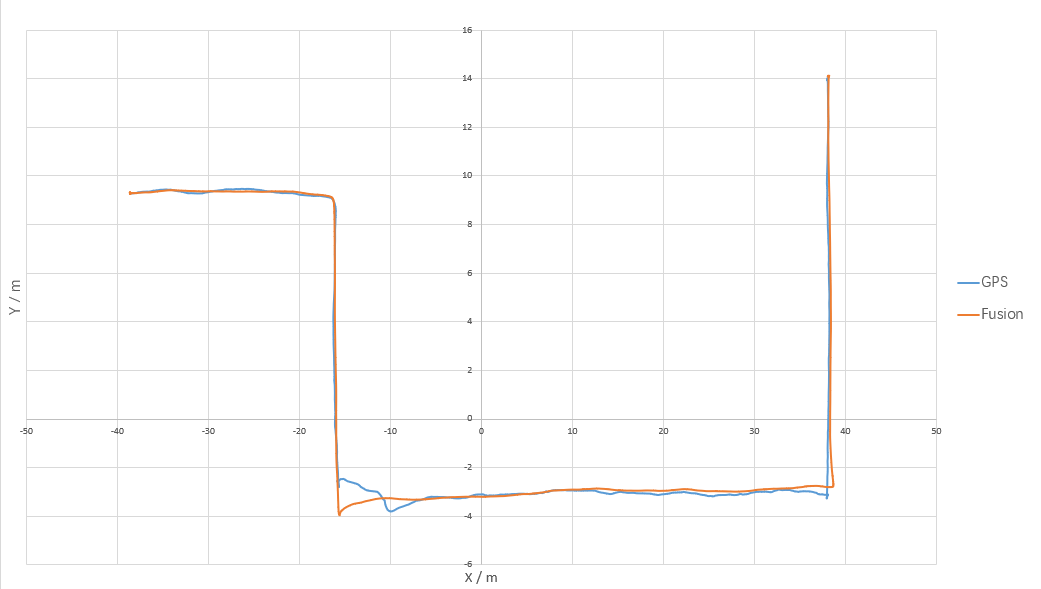
\includegraphics[width=5.76806in,height=3.26333in]{figures/chapter04/卡尔曼融合定位结果.png}
\caption{卡尔曼融合定位效果图}
\label{卡尔曼融合定位效果图}
\end{figure}

室内外定位切换效果如图\ref{室内室外切换效果图}所示。红色轨迹为GPS原始轨迹，黄色轨迹为融合结果。a）时刻车辆在室外运行，GPS略有波动但融合轨迹保持平稳；b）时刻车辆进入室内，GPS信号丢失后系统依靠IMU和轮速计继续定位，轨迹依然平稳。

\begin{figure}[htbp]
\centering
\subfigure[室内环境]{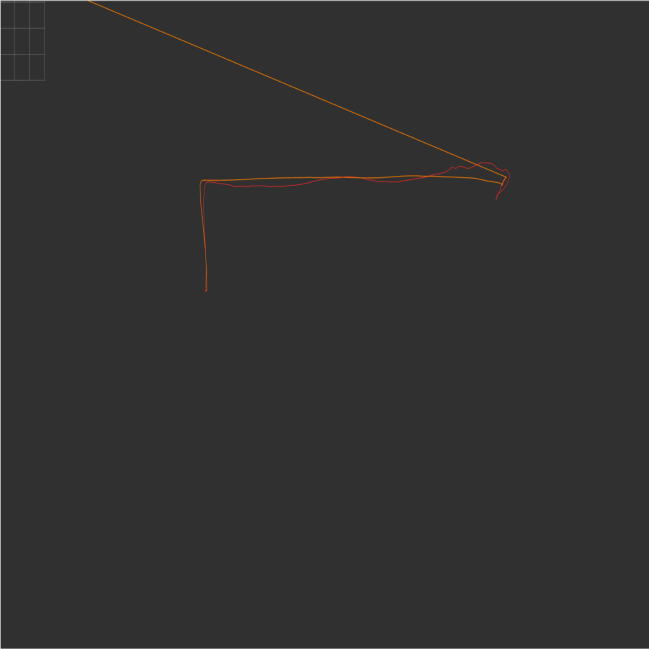
\includegraphics[width=0.44\textwidth]{figures/chapter04/室内环境切换结果.png}}
\hfill
\subfigure[室外环境]{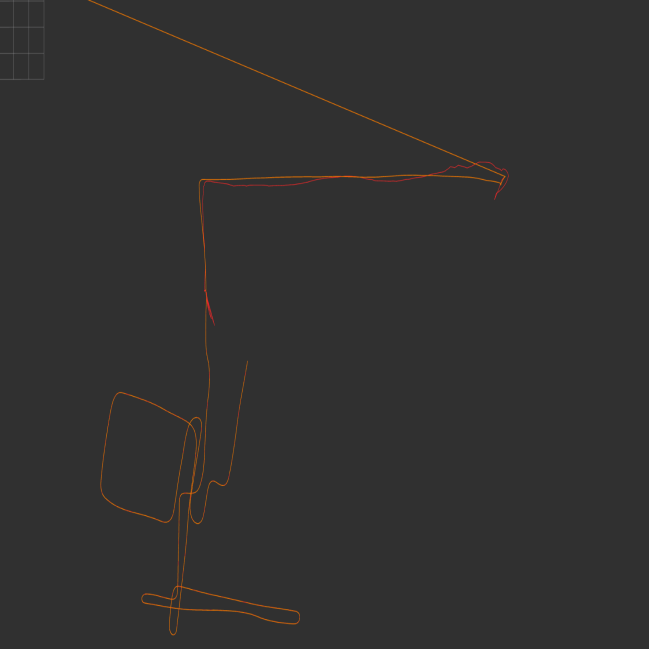
\includegraphics[width=0.44\textwidth]{figures/chapter04/室外环境切换结果.png}}
\caption{室内室外切换效果图}
\label{室内室外切换效果图}
\end{figure}

\subsection{导航模块设计}

在本系统中，导航功能基于ROS中的Navigation框架构建。Navigation框架是ROS官方提供的标准导航解决方案，广泛应用于移动机器人领域，能够实现路径规划、运动控制、定位和障碍物避让等核心功能。该框架提供了良好的模块化结构，便于与各类传感器、地图服务、控制系统集成，适用于本课题中对自主行驶与路径跟踪的需求。

Navigation框架的核心组成包括：地图服务器（map\_server）、定位模块、路径规划模块（global\_planner与local\_planner）、代价地图（costmap\_2d）、运动控制模块（move\_base）等。其中，move\_base节点作为调度中心，协调传感器数据、地图信息、路径规划与底层控制之间的交互。

\subsubsection{导航模块的设计}

导航模块的核心基于ROS中的Navigation导航框架构建，实现从目标接收、路径规划到运动指令输出的全过程。该模块由地图服务、全局规划器、局部规划器、代价地图、坐标变换系统与通信接口等部分组成，各子模块通过ROS话题和服务机制协同运行，如图\ref{导航模块功能结构图}所示。

导航模块从地图模块获取静态环境地图信息，通过map\_server加载至地图服务，为全局路径规划提供环境基础；从定位模块获取实时位姿数据，输入至move\_base节点，用于进行路径规划与轨迹跟踪中的位置判断。

坐标转换信息则由ROS的tf（Transform
Library）坐标系统提供。该系统用于维护多坐标系之间的变换关系，包括地图坐标系（map）、里程计坐标系（odom）和机器人本体坐标系（base\_link）等，使导航模块各功能部件在统一空间基准下完成计算。

\begin{figure}[htbp]
\centering
\includesvg[width=5.76806in,height=3.64514in]{figures/chapter04/导航模块功能结构}
\caption{导航模块功能结构图}
\label{导航模块功能结构图}
\end{figure}

代价地图（costmap）用于表示规划与避障所需的空间约束信息。它接收来自地图模块的静态地图和来自感知模块的动态障碍物数据，并通过膨胀算法形成障碍物影响区域。在ROS
Navigation框架中，代价地图采用二维栅格地图表示，分为全局代价地图（global
costmap）与局部代价地图（local
costmap）：全局代价地图主要用于全局路径搜索，构建在静态环境基础上；局部代价地图则实时叠加感知信息，反映当前动态环境，用于实时避障与局部路径调整。

导航模块从交互模块接收导航目标，将其传递给全局规划器（global\_planner）结合全局代价地图生成初始路径；随后由局部规划器（local\_planner）根据当前位姿和局部代价地图对路径进行动态调整，并生成速度和角速度指令。

最终，导航模块将局部规划器生成的运动指令传递给通信模块，由其下发至控制系统，完成导航任务的执行。

\subsubsection{导航任务的流程}

导航任务的执行流程如图\ref{导航任务流程图}所示，可概括为以下几个阶段：

首先，在系统启动后，导航模块初始化各子模块，包括地图服务、代价地图、规划器、坐标变换系统等，确保其正常运行并完成ROS话题与服务的绑定关系。随后，从地图模块加载静态地图数据，构建用于全局路径规划的环境基础。

导航任务开始后，导航模块从交互模块接收用户或上位系统设定的目标点信息，并通过tf坐标变换系统将目标转换为统一坐标系下的空间位置。随后，从定位模块实时获取机器人当前位姿，并持续更新至导航框架。

\begin{figure}[htbp]
\centering
\includesvg[width=5.76806in,height=5.57917in]{figures/chapter04/导航任务流程图}
\caption{导航任务流程图}
\label{导航任务流程图}
\end{figure}

同时，导航模块从感知模块获取动态环境信息，包括前方障碍物位置与可通行区域，并实时更新至局部代价地图中。这一信息对局部路径规划的有效性和安全性具有重要影响。

一旦目标和当前位姿信息就绪，导航模块触发全局规划器执行一次全局路径规划，生成一条从当前位置到目标点的初始路径。该规划通常在接收到新目标或路径失效时重新计算，不具备周期性。

在全局路径生成后，局部规划器开始以固定周期（如10
Hz）运行，实时结合当前位姿、局部代价地图与全局路径，生成即时控制指令（线速度与角速度）。该指令随后通过通信模块发送至下位控制系统，用于控制底层电机运动。

在导航过程中，导航模块持续判断机器人是否接近设定目标点。若判断到达条件满足（如距离目标点小于设定阈值），则导航模块停止路径追踪过程并输出任务完成信号。

为增强系统在复杂动态环境中的鲁棒性，导航模块还集成了恢复机制。当局部规划器在若干周期内连续规划失败（例如路径被障碍物完全阻断、机器人陷入死胡同或陷入震荡）时，系统将触发一系列预设的恢复行为，这些行为包括：

\begin{itemize}
\item
  清除局部代价地图：用于移除传感器误判导致的局部障碍。
\item
  退后运动：尝试摆脱局部困境或调整朝向。
\item
  原地旋转寻找可行方向：重构局部路径。
\item
  重新全局规划：若原路径长期无效，重新规划全局路径以避开阻塞区域。
\end{itemize}

恢复行为通常按照配置顺序依次尝试，若连续恢复失败仍无法获得可行路径，导航模块将判定导航失败，并可根据需要通知上位系统或进入安全停机状态。

\subsubsection{全局规划}

全局规划器负责在静态环境地图中生成一条从当前位置到目标点的可行路径，路径需避开障碍物并具有一定的平滑性与可达性。其核心任务是基于栅格代价地图进行图搜索路径规划，常见算法包括Dijkstra算法、A*
算法及其变种。

Dijkstra算法是经典的单源最短路径算法，以广度优先方式搜索，逐层扩展路径，通过累计路径代价寻找从起点到终点的最小代价路径。其优点在于路径稳定、可靠性高，能保证在已知代价图中找到一条全局最优路径；缺点是计算效率较低，尤其在大地图中搜索速度慢，且路径往往偏向网格中心，缺乏自然流畅性。

A*算法在Dijkstra基础上引入启发函数，通过估计当前节点到目标点的代价加快搜索过程。其搜索效率更高、路径更自然，适合大规模环境的实时路径规划；但路径质量受启发函数影响较大，若代价估计不当，可能出现较大偏差。

本系统采用ROS\_Navigation框架中的navfn插件，选用Dijkstra算法作为全局路径规划方法。考虑到车行驶速度较低、对路径平稳性要求较高，Dijkstra
能提供更为连贯、确定的路径结果，便于后续的局部优化与跟踪控制。


\begin{table}[htbp]
\centering
\caption{全局规划器的主要参数设置}
\begin{tabularx}{0.9\textwidth}{@{}lXc@{}}
\toprule
\textbf{参数} & \textbf{含义} & \textbf{值} \\
\midrule
base\_global\_planner & 选择规划器插件 & navfn/NavfnROS \\
planner\_patience & 最大规划等待时间（秒） & 5.0 \\
default\_tolerance & 目标点搜索容差半径（米） & 0.5 \\
allow\_unknown & 是否允许穿越未知区域 & false \\
\bottomrule
\end{tabularx}
\end{table}

\subsubsection{局部规划}

局部规划器的任务是基于当前机器人位姿、全局路径以及动态环境信息，生成短期内的可执行运动指令。局部规划器运行于固定周期内，能够动态避障、处理路径扰动，是实现闭环控制的核心组件。典型局部规划方法包括
DWA（Dynamic Window Approach）和TEB（Timed Elastic Band）等。

DWA算法基于机器人动力学模型，首先在速度空间内采样所有可达速度组合，预测在短时间内的轨迹，再结合目标导向性、障碍物距离、速度等多项评价函数选出最优轨迹。其优点是实现简单、运行高效，适用于速度限制严格的差速机器人；缺点是路径受限于速度空间采样，难以产生高质量平滑轨迹，且在复杂环境中可能陷入局部最优。

TEB算法将路径看作一系列时间约束节点组成的弹性带（band），通过最优化方法同时调整路径点的位置和通过时间，从而生成符合运动学约束、避障要求和平滑性的最优路径。TEB特别适合非完整约束平台（如差速驱动机器人），可实现高质量的局部轨迹优化，适用于动态环境下的复杂避障与路径跟踪任务。

综合比较，本系统采用TEB算法作为局部规划方法，并部署于ROS的\texttt{teb\_local\_planner}插件中。该方法适应性强、轨迹自然、避障效果好，适合本系统所需的平稳、安全、实时导航需求。


\begin{table}[htbp]
\centering
\caption{局部规划器主要参数设置}
\begin{tabularx}{0.9\textwidth}{@{}lXc@{}}
\toprule
\textbf{参数} & \textbf{含义} & \textbf{值} \\
\midrule
base\_local\_planner & 局部规划器插件 & TebLocalPlannerROS \\
max\_vel\_x / acc\_lim\_x & 最大前进速度 / 加速度 & 0.8 / 1.0 \\
max\_vel\_theta / acc\_lim\_theta & 最大角速度 / 加速度 & 1.0 / 2.0 \\
min\_obstacle\_dist & 与障碍物最小距离 & 0.3 \\
global\_plan\_overwrite\_orientation & 是否沿用全局路径方向作为参考 & true \\
include\_costmap\_obstacles & 是否纳入代价地图障碍物信息 & true \\
\bottomrule
\end{tabularx}
\end{table}

规划效果如图\ref{导航规划效果}所示，黑色方框为平衡车位置及外边框，黑色长线为全局规划Dijkstra算法所得路径，红色箭头为局部规划TEB算法的一系列局部路径点。

\begin{figure}[htbp]
\centering
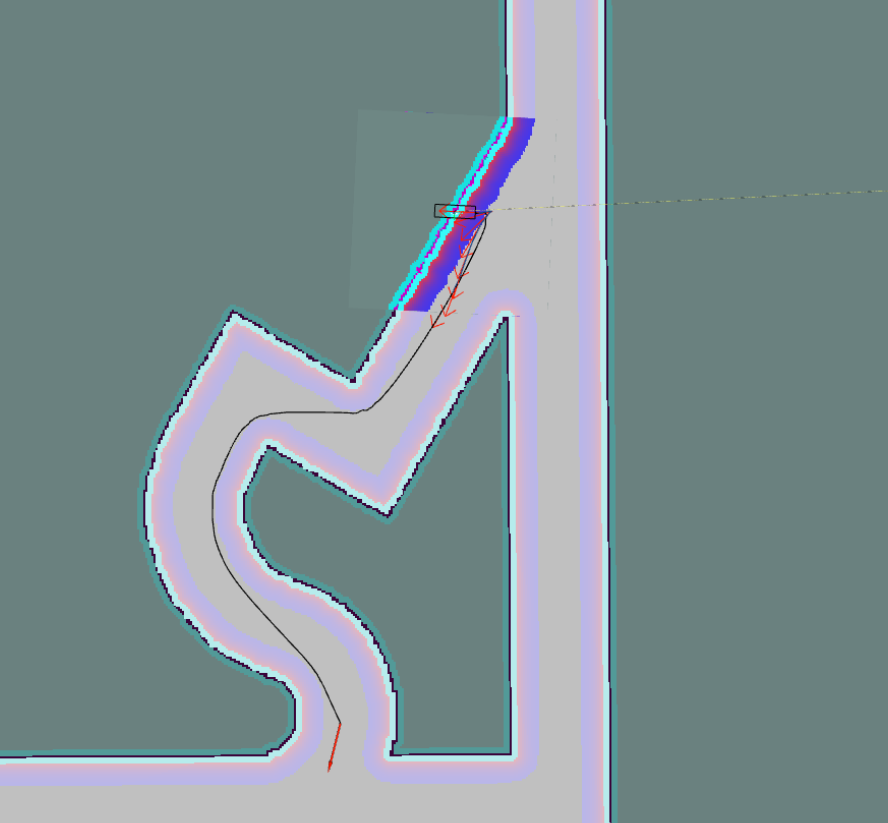
\includegraphics[width=2.99948in,height=2.77991in]{figures/chapter04/导航规划结果.png}
\caption{导航规划效果}
\label{导航规划效果}
\end{figure}

\subsection{感知模块}

感知模块是系统进行环境感知与障碍物检测的核心。本节首先介绍双目相机数据处理流程，然后说明双目相机输出的感知信息如何融合到导航模块中。

双目相机数据处理流程如图\ref{双目相机数据处理流程图}所示。系统首先完成双目相机初始化，包括加载驱动、配置分辨率/帧率/曝光等采集参数，并完成左右摄像头同步设置，以确保后续图像在时间与空间上的一致性。同时，载入相机标定参数，包括内参矩阵、畸变系数及左右相机间外参，用于支持后续立体校正与深度计算。

随后进入循环处理阶段。每轮循环开始时，系统先判断是否达到设定检测周期；若满足条件，则执行一次完整的数据采集与处理。首先获取左右双目图像，再将图像分别送入立体匹配模块和目标检测模块并行处理。

立体匹配模块输出视差图，并基于相机内参转换为深度图。深度图与YOLO目标检测结果结合后，可计算目标空间位置并提取带位置信息的障碍物列表。同时，深度图还用于构建稠密点云，描述当前帧的三维环境信息。最终，系统向核心模块输出该帧障碍物列表及对应环境点云。

\begin{figure}[htbp]
\centering
\includesvg[width=3.51042in,height=4.90625in]{figures/chapter04/双目相机数据处理流程图}
\caption{双目相机数据处理流程图}
\label{双目相机数据处理流程图}
\end{figure}

\subsubsection{障碍物列表在代价地图上的映射}

为了实现对动态障碍物的有效避让，本系统中感知模块将识别出的障碍物以列表形式发布给导航模块。导航模块需将障碍物信息实时映射至局部代价地图，以影响局部路径规划的代价函数，使局部规划器在路径优化过程中主动远离障碍物区域。

代价地图映射采用人工势场（Artificial Potential
Field）中斥力场（Repulsive
Field）的思想，对每一个障碍物位置施加以该点为中心的二维高斯函数，构建空间上的软约束代价分布。其数学表达式如下：
\begin{equation}
C(x,y) = A \cdot \exp\left( - \frac{(x - x_{0})^{2} + (y - y_{0})^{2}}{2\sigma^{2}} \right)
\end{equation}

式中 \emph{C}(\emph{x}, \emph{y})------地图上点(\emph{x},
\emph{y})的代价值；

(x\textsubscript{0}, y\textsubscript{0})------障碍物在地图上的中心坐标；

\emph{A}------高斯函数的振幅，即障碍物中心的最大代价；

\emph{σ}------协方差，控制代价衰减的快慢，值越大则扩散越广；

{\def\LTcaptype{table} % do not increment counter
\begin{longtable}[]{@{}
  >{\raggedright\arraybackslash}p{(\linewidth - 6\tabcolsep) * \real{0.0858}}
  >{\raggedright\arraybackslash}p{(\linewidth - 6\tabcolsep) * \real{0.1154}}
  >{\raggedright\arraybackslash}p{(\linewidth - 6\tabcolsep) * \real{0.2019}}
  >{\raggedright\arraybackslash}p{(\linewidth - 6\tabcolsep) * \real{0.3052}}@{}}
\caption{不同类别障碍物的取值}\label{不同类别障碍物取值}\\
\toprule\noalign{}
\begin{minipage}[b]{\linewidth}\raggedright
类别
\end{minipage} & \begin{minipage}[b]{\linewidth}\raggedright
振幅\emph{A}
\end{minipage} & \begin{minipage}[b]{\linewidth}\raggedright
基础协方差\emph{σ}\textsubscript{base}
\end{minipage} & \begin{minipage}[b]{\linewidth}\raggedright
说明
\end{minipage} \\
\midrule\noalign{}
\endhead
\bottomrule\noalign{}
\endlastfoot
行人 & 255 & 0.5 & 高危险，小但需强烈避让 \\
车辆 & 255 & 0.6 & 体积大，影响广泛 \\
其他 & 200 & 0.25 & 中等影响 \\
\end{longtable}
}

为兼顾识别精度与运行效率，系统采用基于障碍物类别的代价参数设定机制。在实现时，导航模块从障碍物列表中读取每个障碍物的分类标签（由YOLO输出的class\_id）。系统首先根据表\ref{不同类别障碍物取值}按类别确定振幅\emph{A}和基础协方差\emph{σ}\textsubscript{base}，然后引入其实际宽度\emph{w}，通过如下方式计算最终协方差：
\begin{equation}
\sigma=\sigma_{\text{base}}\cdot w
\end{equation}

这样可保证危险级别高或体积较大的障碍物在代价地图上形成更广的影响区域，增强避障保守性；而小型目标则仅形成局部约束，避免对路径规划造成过多干扰。

障碍物列表在代价地图中的映射流程如下：首先读取障碍物的分类标签与几何宽度；再查表确定振幅\emph{A}和基础协方差\emph{σ}\textsubscript{base}，计算\emph{σ}=\emph{σ}\textsubscript{base}·\emph{w}；随后使用高斯函数计算周围栅格代价值；最后对所有代价值大于截止值的栅格更新局部代价地图。

障碍物列表在代价地图上的映射效果如图\ref{障碍物列表在代价地图上的映射}所示。

\begin{figure}[htbp]
\centering
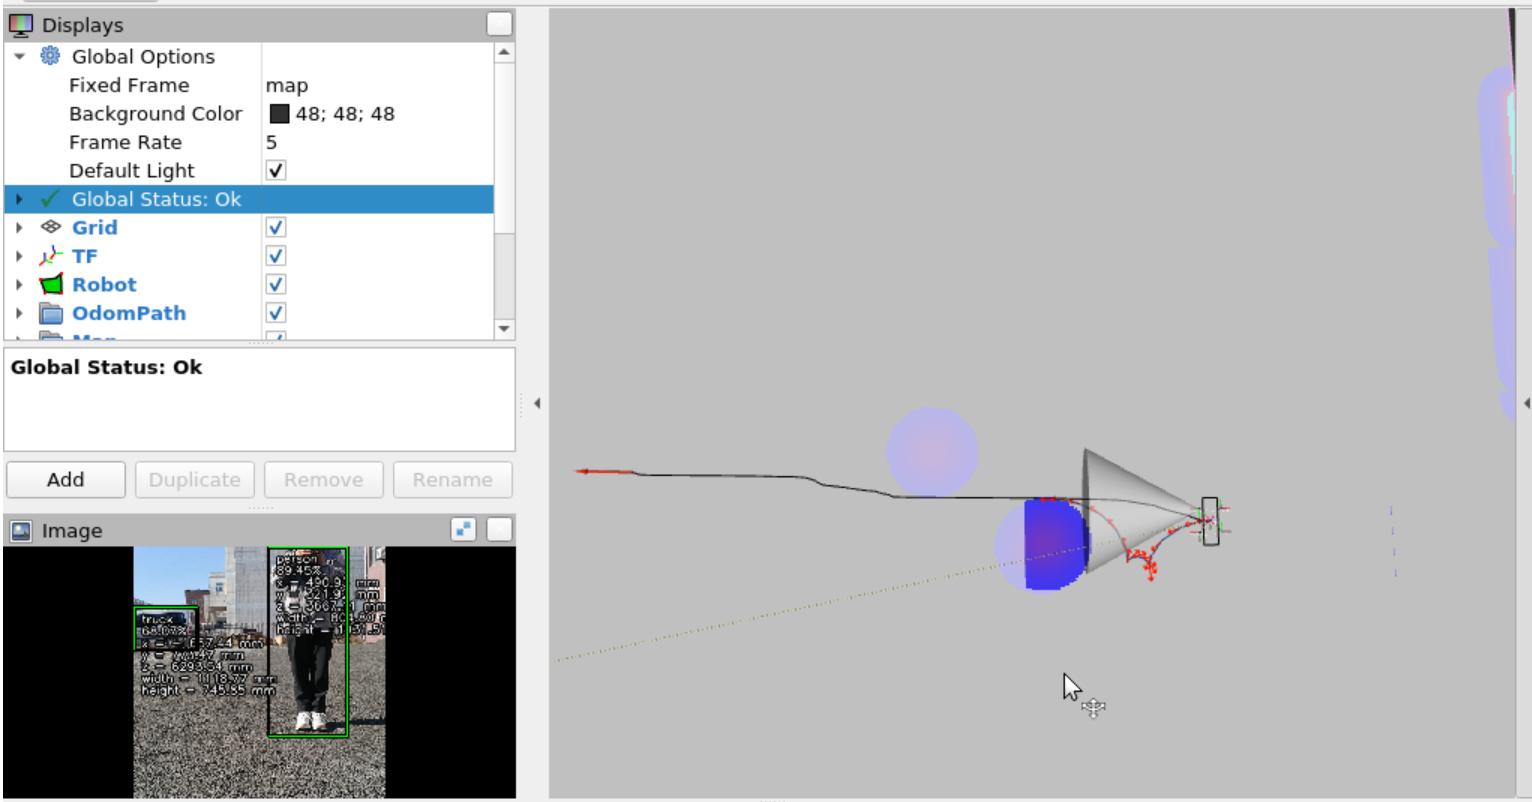
\includegraphics[width=5.42456in,height=3.24716in]{figures/chapter04/障碍物列表代价地图映射.png}
\caption{障碍物列表在代价地图上的映射}
\label{障碍物列表在代价地图上的映射}
\end{figure}

\subsubsection{环境点云在代价地图上的映射}

为实现对非特定障碍物的检测与规避，系统将实时获取的点云数据映射至代价地图。在映射前，需对原始点云进行空间滤波，剔除无效或冗余信息。具体做法是设定距离阈值与高度阈值，滤除位于感知范围之外（如距离过远）或高度不符合障碍物特征（如低于地面或高于平衡车可通过高度）的点云数据。

考虑到两轮平衡车仅在平面内运动，因此仅需分析二维平面(x,y)上的空间占据情况。遍历过滤后的点云数据，对每一个(x,y)平面位置，若其垂直方向z上存在任意点（即该处存在物体），则认为该点为不可通行区域。此类点在代价地图中赋予最大代价值（255），以表示完全障碍，确保规划系统在路径搜索时绕开该区域。环境点云在代价地图上的映射效果如图\ref{环境点云在代价地图上的映射}所示。

\begin{figure}[htbp]
\centering
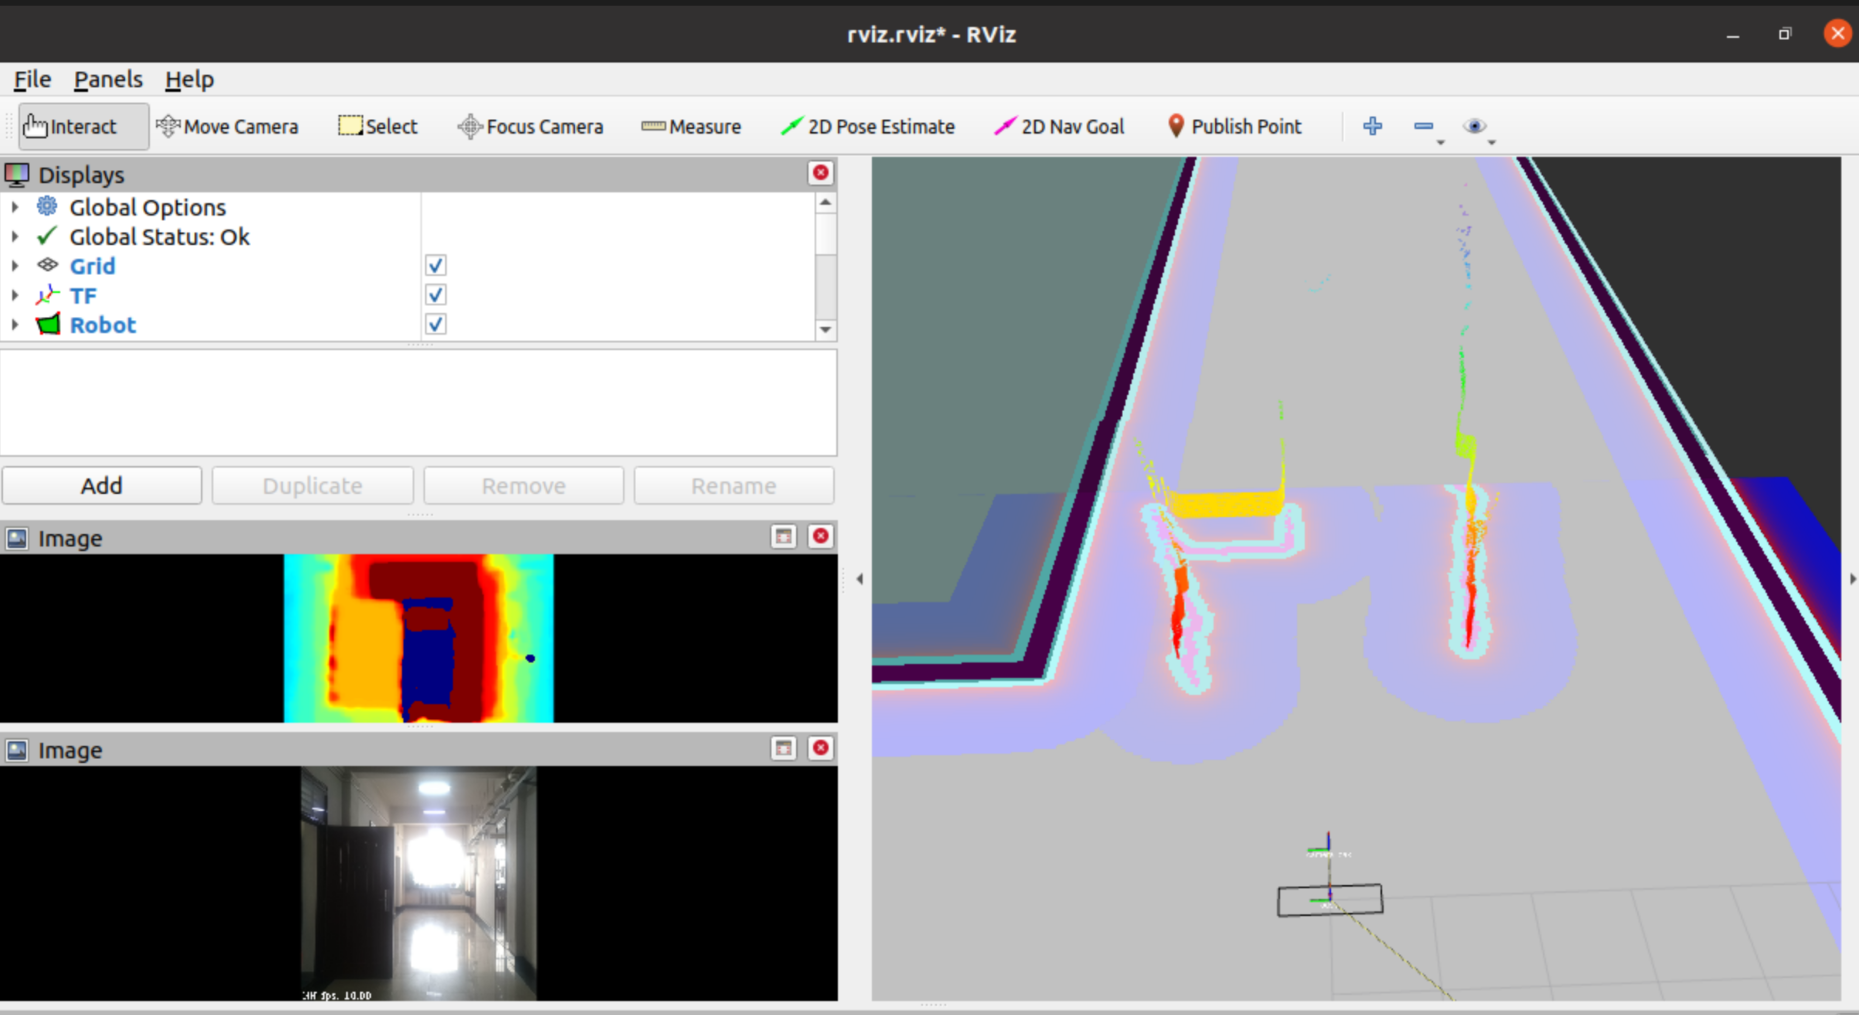
\includegraphics[width=5.53914in,height=3.02432in]{figures/chapter04/点云代价地图映射.png}
\caption{环境点云在代价地图上的映射}
\label{环境点云在代价地图上的映射}
\end{figure}

\section{本章小结}

本章围绕两轮平衡车自主导航需求，完成了系统总体架构设计、软硬件平台搭建及核心功能实现。系统构建了包含定位、感知与路径规划的导航框架，明确了各模块的数据流与控制关系，形成感知、决策、控制闭环。硬件方面，完成主控平台、双目相机、IMU及底盘控制单元的集成与接口配置，保障系统稳定运行。软件方面，基于ROS搭建总体架构：定位模块实现多源信息融合与位姿估计，导航模块完成路径规划与局部避障，感知模块输出目标检测与距离信息，各模块通过标准话题接口实现解耦协同。本章完成了自主导航系统的集成实现，为整车实验与性能验证提供了系统基础。




